\chapter{Umsetzung}
\label{chapter:Umsetzung}

In den folgenden Abschnitten wird auf die Umsetzung der Anwendung und des KNN eingegangen.

\section{Umsetzung der Anwendung}
\label{section:Umsetzung der Anwendung}

\subsection{Oberfläche}
\label{subsection:Oberfläche}

\begin{figure}
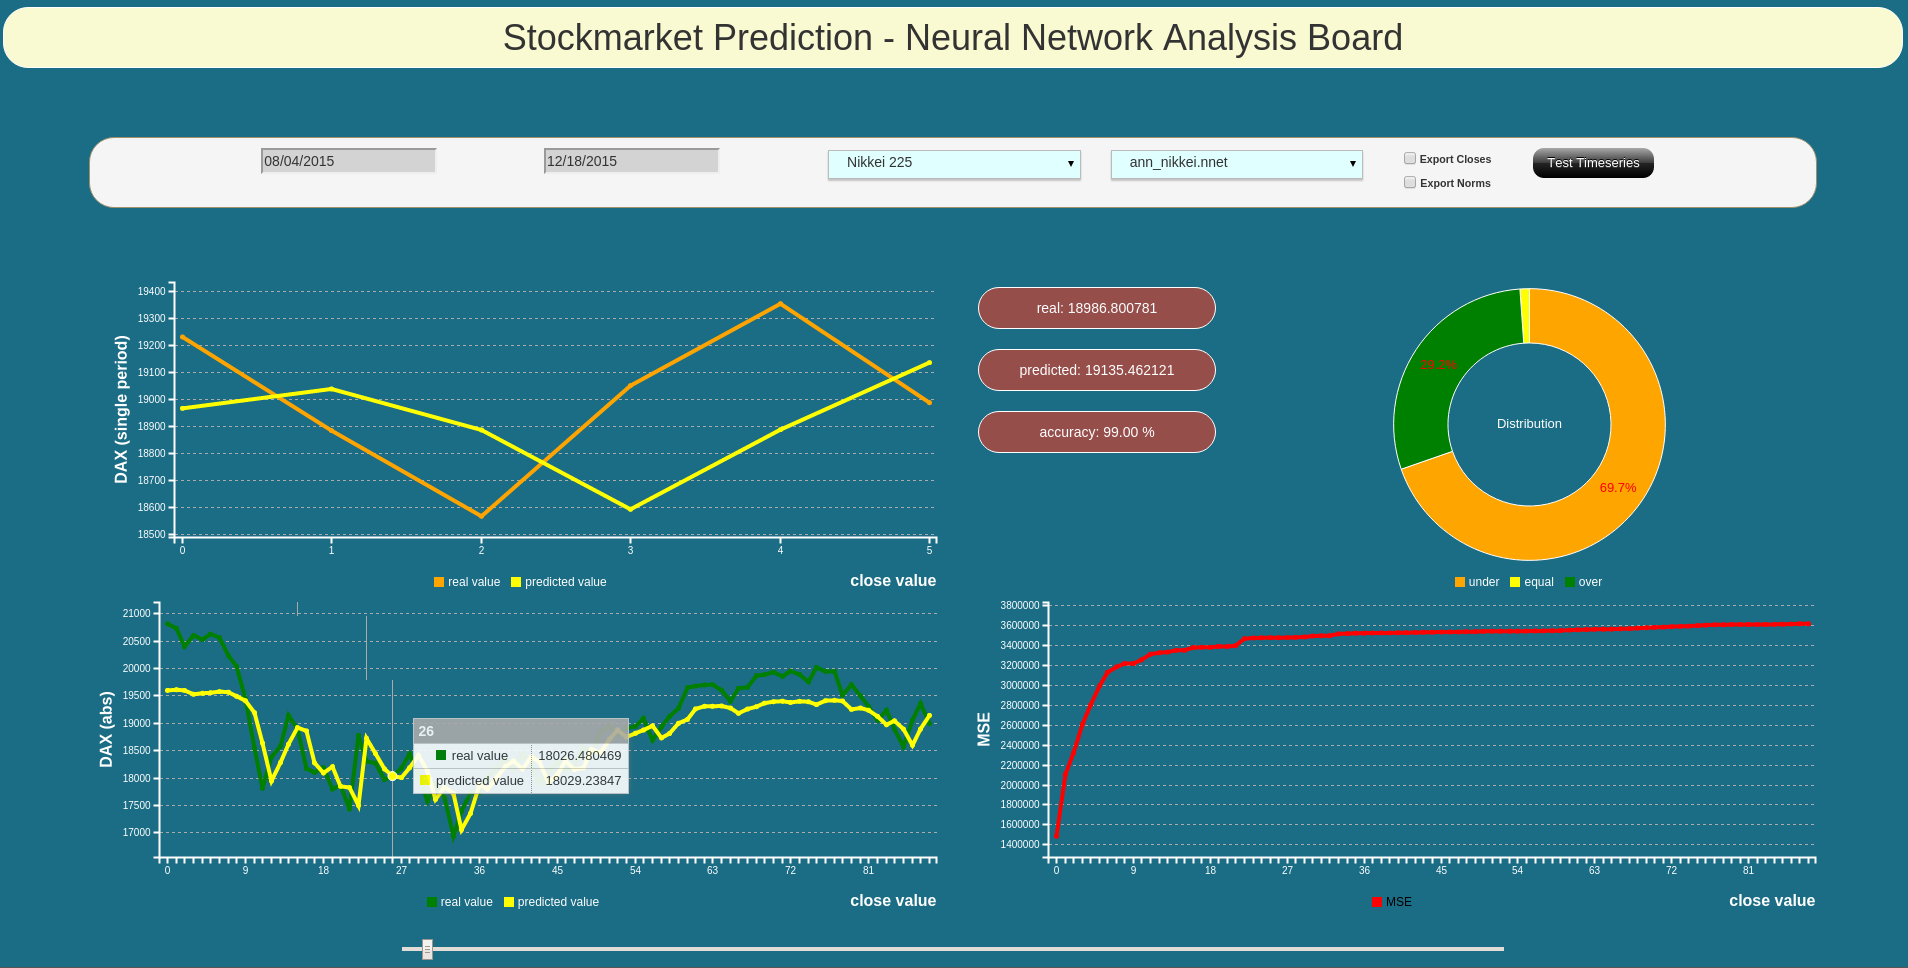
\includegraphics[width=15cm]{Bilder/Umsetzung/Mokup_GUI.png}
\end{figure}
Die Oberfläche ist grob eingeteilt in zwei funktional getrennte Bereiche. Der weiße Container beinhaltet ein Formular das der Anfragestellung dient. Hierin werden die Rahmenbedingung der Vorhersage eingegeben. Zum einen Start - und Enddatum, sowie welche Datenmengen, die von Quandl bezogen werden mit welchem Neuronalen Netz getestet werden sollen. Sofern die davon rechts gelegenen Checkboxen angeklickt abgeschickt werden, so werden CSV-Datein mit den entsprechenden Rahmenbedingung in einem konfigurierbarem Verzeichnis gespeichert. \emph{Export Closes} steht hierbei für denormalisierte Börsenschlusswerte, \emph{Export Norms} für die gleichen normalisierten Werte. Mit \emph{Test Timeseries} werden alle Informationen serialisiert und die Anfrage durchgeführt.\\
Das Ergebnis der Anfrage wird, sofern sie die Fehlerprüfung übersteht, unterhalb des Formulars angezeigt. Die Ausgewählten Werte bleiben hierbei dem Formular hinterlegt.
Die Antwort wird in Form von Diagrammen und Displays angezeigt. Alle Informationen werden bzgl. eines zeitlichen Intervalls aktualisiert, somit wird eine Art Echtzeit-Darstellung realisiert.\\ 
Die Javascript Bibliothek \emph{C3js} wird bei der Realisierung von vier Diagrammen eingesetzt. Das erste links oben angeordnete visualisiert diskrete \emph{tatsächliche} Werte (real value) und \emph{vorhergesagte Werte} (predicted value) für einen definierten Zeitraum \emph{single period}. Dies dient vor allem der Übersicht, so wird eine Art \emph{Zoom}-Modus realisiert. Das zweite unten links angeordnete Diagramm visualisiert die gleichen Werte, jedoch über den gesamten Zeitraum \emph{absolute-graph} dar, was einem Resümee bzgl. der Vorhersage zuträglich ist.\\
Das dritte und letzte Diagramm stellt den Mean-Square-Error-Graph (MSE) der gesamten Zeitreihe dar. Die erste drei Diagramme sind vom gleichen Typ. 
Eine weitere statistische Auswertung, die oben rechts also c3-donut-Diagramm umgesetzt ist, ist die Klassen-Zuordnung von vorhergesagten Werten in die Klassen \emph{under} (unterhalb vom tatsächlichen Wert), \emph{equal} und \emph{over}. Da in der Realität die Werte fast nie exakt übereinstimmen, wurde ein Konfidenz-Intervall definiert, dass eine gewisse Fehlertoleranz gegenüber der Differenz beider Werte zulässt und equal-Klasse somit faktisch keine leere Menge bildet. \\
Des weiteren wurden Displays mit eigens geschriebenem CSS-Klassen definiert, die den tatsächliche, den vorhergesagten sowie die \emph{accurancy} (Exaktheit) Anzeigt. Die Accuracy lässt sich als Betrag der Differenz zweier Werte verstehen. \\
Am unteren Rand ist ein Schieberegler integriert um die Echtzeit-Intervalllänge zu verändern.\\\\


Im folgenden wird ein Anfrage-Antwort-Zyklus (Request-Response-Lifecycle) der Umsetzung detailliert beschrieben und erläutert, welche Rolle die bereits vorgestellten Technologien und Überlegungen in die Implementierung eingeflossen sind, sowie wie diese miteinander verknüpft sind.      

\subsection{Dataset und AnnNames ajax}
\label{subsection:Dataset und AnnNames ajax}
Die Auswahl der Quandl-Datensätze, sowie der .nnet-Datei werden ausschließlich mit Hilfe der Stockmarket-Webapp befüllt. Hierbei werden die Informationen mit AJAX-Aufrufen abgefragt. 

\subsection{Anfrage}
\label{subsection:Anfrage}

\subsection{Anfragestellung}
Das Auslösen einer Anfrage wurde bereits oben geschildert. Der Button-Click wird mit einem jQuery-Event-Listener behandelt. Dieser führt eine Fehlerprüfung der Formulareingabe durch. Wenn ein Enddatum eingegeben wird, dass kleiner dem Startdatum ist, so wird eine entsprechende Fehlermeldung in einem \emph{div}-Tag geladen. Gleiches passiert das, wenn unvollständige Angaben gemacht werden.\\
Beim Bestehen der Prüfung wird ein AJAX-Aufruf (Asynchronous JavaScript and XML) für den ReSTController der Stockmarket-Webapp ausgeführt. Hierbei wird eine URI konstruiert, die zum einen die Basis-URL des Webservice anspricht, zum anderen die  Formulareingabedaten als Parameter enthält. Wenn der Aufruf erfolgreich durchgeführt wird, werden die Hilfsvariablen im Javascript der Visualisierung erneut initialisiert, damit es bei mehreren hintereinander folgenden Ausführungen ohne Seitenaktualisierung keine veränderte Verarbeitungsroutine der Antwortdaten gibt.

\subsection{Antwort-Erstellung}
Die Antwort-Erstellung obliegt der Stockmarket-Webapp, die Visualisierung liefert die Eingabedaten hierzu. Der ReSTController ist das Verbindungsglied im Anfrage-Antwort-Lebenszyklus, aber auch die Komponente, die die Programmablauflogik der Antworterstellung implementiert. Dieser enthält drei Rest-Endpunkte, entsprechend der drei Anfragen, die die Visualisierung per AJAX realisiert.\\

\begin{lstlisting}[basicstyle=\scriptsize, caption=ReSTController Snippet]
@RestController
@RequestMapping(value = "/stock")
public class ReSTController implements ServletContextAware, ServletConfigAware {

    @Autowired
    private EnvService envService;

    @Autowired
    private DataService dataService;
    
    \vdots
    
    @RequestMapping(value= "/data", method = RequestMethod.GET)
    public String data(@RequestParam String startDate,
                       @RequestParam String endDate,
                       @RequestParam String collapse,
                       @RequestParam String stock,
                       @RequestParam String ann,
                       @RequestParam Boolean saveNorm,
                       @RequestParam Boolean saveClose ) 
                       {
	// Programmablauflogik
	\vdots
	}

   @RequestMapping(value= "/ann_names", method = RequestMethod.GET)
   public List<String> annNames()
   {    
   \vdots
   }
    
   @RequestMapping(value= "/datasets", method = RequestMethod.GET)
   public String datasets() 
   {
   \vdots
   }
}    
    
\end{lstlisting}   

Die ReSTController-Klasse ist mit \emph{@RestController} annotiert, was eine Implementierung der \emph{ServletContextAware} und \emph{ServletConfigAware} erfordert. Diese stellen sicher, dass der ReSTController auf den Servlet-Kontext zurückgreifen kann sowie die Servlet-Konfiguration beachtet wird. Diese wird unter anderem dazu verwendet, die Basis-URL zu spezifizieren.\\
Die Rest-Endpunkte werden relativ zu dieser Basis-URL abgebildet. Die Annotation \emph{@RequestMapping} erlaubt die Kennzeichnung von Klassen und Methoden als Zielpunkte gleichermaßen. Entsprechend der HTTP-Verbs können Anfrage-Methoden (RequestMethod) spezifiziert werden. Für den ReSTController wird ein Basis-Endpunkt \emph{/stock} definiert.\\  
Das \emph{data}-Methode implementiert die Programmlogik für die Antworterstellung, die annNames-Methode liest die Bezeichnungen der .nnet-Dateien, die \emph{datasets}-Methode die Rest-Endpunkte der Quandl-Datasets zu den entsprechenden Börsenkursen aus der \emph{app.properties} Datei.\\
Die URI des AJAX-Aufruf des Eingabeformulars wird in der Methodensignatur auf Vollständigkeit und Datentyp-Korrektheit mit der \emph{@RequestParam}-Annotation überprüft. \emph{@RequestParam} fordert einen URL-Parameter gleichnamig zum Variablennamen zu übergeben, alternativ könnte man eine \emph{@Param}-Annoation verwenden, die eine unterschiedliche Namensgebung erlaubt, und sich an der Reihenfolge der Parameter orientiert. \\
Die Antworterstellung ist auf sechs Serviceklassen aufgeteilt, die wiederum gekapselt in einer Serviceklasse sind. Der ReSTController bindet ausschließlich den diese Klasse, den \emph{Data-Service} ein.\\
Erster Schritt ist das Einlesen einiger Konfigurationseigenschaften aus der \emph{app.properties}-Datei. Unter anderem das gewünschte Rückgabeformat des Quandl-Datasets sowie die Basis-URL der Quandl-API. Anschließend wird wird aus den zur Vefügung stehenden Informationen eine URI konstruiert und eine Restabfrage der Quandl-Api durchgeführt. Das Ergebnis wird als Liste von Zeichenketten gespeichert.  
Dabei wird die Daten mit folgenden Spezifikationen angefragt:
 
 
 \begin{table}
  \centering
  \begin{tabular}{lll}   
    Quandl-API URL-Parameter & Bedeutung \\
    \midrule
   
    \tabitem order & Reihenfolge der Ergebnismenge  \\
    \tabitem exclude\_column\_names & Schließt Header-Information aus \\  
    \tabitem start\_date & Startdatum \\   
    \tabitem end\_date & Enddatum \\
    \tabitem collapse & Datenfequenz\\
    \bottomrule
  \end{tabular}
  \caption{verwendete URL-Parameter - Quandl API}
\end{table}



Der zweite von zehn Methodenaufrufen, die der \emph{data-Service} organisiert ist das Formatieren der Ergebnismenge in eine für die Neuroph-API passende Struktur. Diese Aufgabe übernimmt der FormService.

% \begin{table}
%  \centering
%  \begin{tabular}{lll} 
%    Date & Open & High & Low & Close & Volume & Adjusted Close \\
%    \midrule              
%    \tabitem 2015-01-02 & 17823.07 & 17951.78 & 17731.3 & 17832.99 & 76270000.0 & 17832.99 \\
%	\tabitem 2015-01-05 & 17821.3 & 17821.3 & 17475.93 & 17501.65 & 116160000.0 & 17501.65 \\
%	\tabitem 2015-01-06 & 17504.18 & 17581.05 & 17262.37 & 17371.64 & 101870000.0 & 17371.64 \\
%	\tabitem 2015-01-07 & 17374.78 & 17597.08 & 17374.78 & 17584.52 & 91030000.0 & 17584.52 \\
%	\tabitem 2015-01-08 & 17591.97 & 17916.04 & 17591.97 & 17907.87 & 114890000.0 & 17907.87 \\ 
%    \bottomrule
%  \end{tabular}
%  \caption{Beispielantwort - Quandl API}
%\end{table}

%
%  \begin{table}
%  \centering
%  \begin{tabular}{lll}   
%    Date & Close t-4 & Close t-3 & Close t-2 & Close t-1 & Close t \\
%    \midrule            
%    \tabitem 2015-01-08 & 17832.99 & 17501.65 & 17371.64 & 17584.52 & 17907.87 \\
%    \bottomrule
%  \end{tabular}
%  \caption{Formatierte Beispielantwort - Quandl API}
%\end{table}

Die Konversion beachtet zwei Kriterien, zum einen die Anzahl der Input-und Output-Neuronen, die in der Konfigurationsdatei unter der Eigenschaft \emph{format.period.length} also Summe angegeben ist, sowie die Spaltenposition desjenigen Wertes, der vorhergesagt werden soll, also der Börsenschlusswert.
Es werden ausschließlich Börsenschlusswerte und deren Datum berücksichtigt. Eine Zeile in der konvertierten Liste besteht aus dem Datum des letzten (spätesten) betrachteten Wert innerhalb einer Periode, sowie die Werte der gesamten Periode. Das Ergebnis wird als Listen von Listen von Zeichenketten gespeichert, was einen bessere Verarbeitung für die folgenden Schritte ermöglicht.\\\\

Als zweiter Schritt steht die Normalisierung an. Diese Aufgabe wird im \emph{NormDenorm-Service} durchgeführt. Wie in Kapitel 3.3 beschrieben gibt es unterschiedliche Ansätze für die Normalisierungsfunktion, die von der Wahl der Aktivierungsfunktion abhängt. Somit ist es sinnvoll die Formeln für die Normalisierung und Denomalisierung auszulagern um keinen Flaschenhals für künftige Anpassungen oder Experimente zu bilden. Die \emph{normalize-}Methode ließt zuerst die entsprechende Formel, die maximale Anzahl gewünschter Nachkommstellen sowie die Periodenlänge aus der \emph{app.properties} Datei. Die Erfüllbarkeit der Funktion in Kapitel 3.3 hängt von der Möglichkeit ab, das globale Maximum und Minimum zu bestimmen. Damit wird gewährleistet, dass aussschießlich Werte zwischen Null und Eins angenommen werden können. Da unsere Datenmenge eine feste Größe besitzt ist dies kein Problem. 
Eine überaus nützliches Softwarepaket ist der \emph{ScriptEngineManager}, diese die Art der Modularität erlaubt. Dieser kann einen als Javascript initialisierten \emph{ScriptEngine} verwenden um die eingelesene Funktion (Zeichenkette) entsprechen zu interpretieren. Die private Methode \emph{processFormula} wird für Normalisierung und Denormalisierung verwendet. Diese konvertiert schließlich jeden Wert der Liste über die übergebene Funktion. 
Anschließend wird die Liste eine Variable im ReSTController zurückgegeben. \\\\

Die nächsten zwei Schritte setzt die Anfrage der Checkboxen in die Tat um und speichern, sofern im Formular angeklickt, transformierte Börsensschlussdaten sowie normalisierte Daten als CSV-Dateien in ein Verzeichnis, dessen Pfad in der \emph{app.properties}-Datei festgelegt ist. Der Dateinamen ist autogeneriert und besteht aus dem angefragten Zeitraum sowie dem Namen des Datasets. Notwendig war diese Funktionalität vor allem für das Training der Neuronalen Netze, das im Neuroph Studio durchgeführt wurde, also außerhalb der Anwendung. \\\\

Im fünften Schritt wird das Neuronale Netz mit den normalisierten Daten getestet. Der \emph{Ann-Service} implementiert hierzu eine Methode \emph{testAnn}. Um die Erweiterbarkeit auch für künftige Umsetzungen von Neuronalen Netzen möglichst einfach zu gewährleisten, so z.B. eine andere Topologie zu verwenden, die auf mehr Eingangsneuronen setzt, wird die Periodenlänge aus der \emph{app.properties}-Datei gelesen. Der Testalgorithmus wird allgemeingültig gehalten, und funktioniert für alle Neuronalen Netztypen, die ein Ausgangsneuron besitzen. 
An dieser Stelle wird das erste mal die Neuroph-Core-Bibliothek innerhalb der Stockmarket-Webapp verwendet. 
Zuerst wird eine \emph{Dataset}-Instanz mit der Anzahl der Input- und Outputneuronen initialisiert.
Anschließend wird die normalisierte Liste zeilenweise iteriert. Jede Zeile wird in zwei Arrays von \emph{double}-Werten geteilt, ein Input- und Output-Array und anschließend dem DataSet-Objekt hinzugefügt.
Als nächstes wird das Multi-Layer-Perzeptron über den hinterlegten Dateipfad geladen. Hierzu bietet Neuroph die \emph{createFromFile}-Methode.
Anschließend wird das DataSet-Objekt in eine Liste von \emph{DataSetRow}-Instanzen gesplittet. Eine DataSetRow ist das wichtigste Attribut der DataSet-Klasse und repräsentiert einen Testschritt. Für jedes Input-Array in einer solche DataSetRow wird ein Ausgabewert errechnet, welcher zu einer Liste aus Zeichenketten hinzugefügt wird.
Nachdem die Iteration abgeschlossen ist und die Menge der vorhergesagten Werte vollständig kalkuliert wurde, wird die Liste mit der Testdatenliste erweitert. Diese Aufgabe übernimmt der entsprechend \emph{Form-Service}.\\\\

Der sechste Schritt ist die Denormalisierung der gewonnen Ergebnisliste. Wie oben bereits erwähnt wird die \emph{processFormula}-Methode des \emph{NormDenorm-Serive} lediglich mit anderen Parameterwerten ausgeführt. Es wird die Denormalisierungsfunktion, die maximale Anzahl der Nachkommastellen sowie die Periodenlänge aus der \emph{app.properties}-Datei geladen und übergeben. Eine Funktionalität die derzeit nicht benötigt wird, aber dennoch implementiert ist, stellt die Möglichkeit dar Spalten der List von den Operationen auszuschließen. Wären zu diesem Zeitpunkt bereits denormalisierte Werte vorhanden, wäre dies deshalb kein Problem.

Der siebte und letzte Schritt, der eine Modifikation der Liste vollführt ist das hinzufügen von Fehlermaßen. Hierfür ist der \emph{Error-Service} zuständig. Grundidee des Error-Service ist, eine Methode pro Fehlermaß umzusetzen, wobei jede Methode eine Liste von Zeichenketten zurückgibt. Der \emph{Data-Service} greift ausschließlich auf eine im zugedacht Methode zu, die für alle diese Fehlermethoden zuständig ist. Hier ist das die \emph{getAllErrorMessures}-Methode. Als erstes wird geprüft ob ein Fehlermaß überhaupt hinzugefügt werden soll. Diese Informationen sind in der \emph{app.properties}-Datei gelistet. Für jedes Fehlermaß gibt es einen Eintrag mit dem Präfix \emph{error.avail}, der als \emph{Boolean}-Wert interpretiert wird. Je nach dem ob diese wahr sind, werden die entsprechenden Fehlermaße berechnet. Die Ergebnislisten dieser Methoden werden zu einer großen Ergebnisliste hinzugefügt und anschließend mit der \emph{addCols}-Methode des \emph{FormService} hinzugefügt.
Für jedes weitere Fehlermaß muss also lediglich ein Eintrag in der app.properties sowie eine Methoden Implementierung umgesetzt werden, welche in der Hauptmethode entsprechend ausgeführt wird. Somit können die Ziele von Funktionsumfang, Flexibilität und Performance harmonieren.\\
Der Mean-Square-Error (MSE) wird bereits in ..... erklärt. Des Weiteren wird hier die \emph{Accuracy} (Exaktheit) sowie die \emph{Distribution} (Klassenzuteilung) berechnet. Das hierfür benötigt Konfidenzintervall bleibt ebenfalls als Eigenschaft in der Konfigurationsdatei hinterlegt. 

Abschließender Schritt zur Antworterstellung ist die Konversion der generierten Liste in einen geeignete Struktur, damit die Visualisierung eine möglichst einfache Handhabe bei dem Verarbeiten der Daten hat. Die Aufgabe übernimmt sinngemäß der \emph{FormService}. Die Methode \emph{parseResponseList} gibt ein \emph{JSONArray}-Objekt zurück. Dieses wird iterativ befüllt, indem jede Liste innerhalb der Ergebnisliste in einer fest definierte Struktur innerhalb einer jeweils neuen JSONObject-Instanz abgebildet wird. Zu jedem Wert gibt es einen textuellen Schlüssel, somit kann auf einen Schleifendurchlauf eines JSONObjekt innerhalb des Arrays in der Visualisierung verzichtet werden und der entsprechende Wert unmittelbar angesprochen werden. Der \emph{Data-Service} wandelt das JSONArray-Objekt in einen String. Dieser wird der Visualisierung nun als Antwortnachricht übergeben. 


\begin{lstlisting}[basicstyle=\scriptsize, caption=Beispiel - JSONArray]
[  
   {  
      "date":"2015-12-07",
      "acc":"100.00",
      "input":[  
         "11261.240234",
         "11190.019531",
         "10789.240234",
         "10752.099609"
      ],
      "dist":{  
         "equal":"0",
         "over":"0",
         "under":"1"
      },
      "ro":"10886.089844",
      "mse":"454.036617",
      "po":"10864.781709"
   }
]
\end{lstlisting}



\begin{figure}
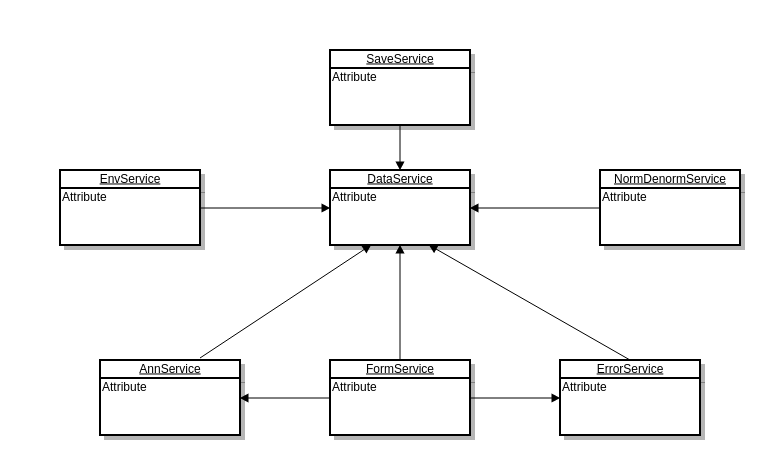
\includegraphics[width=15cm]{Bilder/Umsetzung/sequence_dia_service_layer.png}
\end{figure}


\subsection{Antwort-Verarbeitung}
Die Zeichenkette des JSON-Arrarys wird in einer globalen Variable zwischengespeichert. Da alle Diagramme und Displays einem einheitlichen Takt folgen sollen, wird die Initialisierung der Graphikkomponenten, sowie deren gesamter Aktualisierungszyklen von einer Funktion \emph{setDeceleratingTimeout} aufgerufen. Nach einer Verzögerung, die durch eine globale Intervalllängendefinition beeinflusst wird und über die JavaScript-spezifische Methode \emph{window.setTimeout()} realisiert wird, wird jeweils die \emph{processValues}-Funktion abgearbeitet. In dieser wird jeweils eine JSONObject-Repräsentation verarbeitet und für die Anzeige für das kommende Intervall vorbereitet sowie anschließend an die Darstellungsfunktionen (Rendering-Funktionen) übergeben. Grob gesagt werden entsprechende temporäre Arrays mit den Werten der Repräsentation befüllt und übergeben. Neben den Darstellungen wird der Schieberegler, der den Wert der globalen Variable \emph{Interval} in Echtzeit verändert, in die Visualisierungslandschaft integriert. 

\subsection{Konfigurationsdatei der Stockmarket-Webapp}

\begin{lstlisting}[basicstyle=\scriptsize, caption=app.properties - Konfigurationsdatei der Stockmarket-Webapp]

## filepath where ann files are stored
media.source.base=/home/bthofrichter/Schreibtisch
media.source.ann=/source/ann
media.source.analyzed=/source/analyzed/

quandl.api.baseurl=https://www.quandl.com/api/v3/datasets

quandl.api.key=KsHDYzZK6uyyynwQNS7p

## response format by quandl API
quandl.data.dataset.format=csv
quandl.data.dataset.order=asc
quandl.data.dataset.header=true
quandl.data.dataset.close.pos=4

##
format.period.length=5
format.data.included=true
format.data.norm.precision=12
format.data.denorm.precision=6
format.data.error.acc.precision=2

dist.conf=10

## quandl datasets
quandl.dataset.dax=/YAHOO/INDEX_GDAXI
quandl.dataset.nikkei_225=/YAHOO/INDEX_N225
quandl.dataset.djia=/YAHOO/INDEX_DJI


## quandl dataset names for visualisation
quandl.dataset.name.dax=DAX,dax
quandl.dataset.name.nikkei_225=Nikkei 225,nikkei_225
quandl.dataset.name.djia=Dow Jones (DJIA),djia

## X := current value
## MIN := global minimum
## MAX := global maximum
normalize.formula=((X-MIN)/(MAX-MIN))*0.8+0.1
denormalize.formula=((X-0.1)/0.8)*(MAX-MIN)+MIN

## ERROR-AVAILABILITY
error.avail.dist=true
error.avail.mse=true
error.avail.acc=true
\end{lstlisting}

\subsection{Maven POM der Anwendung}

Die in ListingPOM zeigt die Grundstruktur der POM.xml der Anwendung. Diese enthält alle wichtigen Informationen um die Anwendung in der Beschriebenen Systemlandschaft zu bauen.\\
Kurze Erläuterung zum Aufbau der POM.xml: \\
Project-Knoten: Enthält alle anderen Knoten. Die Deklaration in 
Zeile 1--4 verweist auf eine entsprechende Namensraum und Schema-Defintion. 
modelVersion-Knoten: Die Versionsnummer muss mit den Versionsinformationen im Proect-Knoten übereinstimmen.
In Zeile 7-9 sind die typischen 3 Knoten \emph{groupId}, \emph{artifactId} und \emph{version} zur Beschreibung einer Dependency. Da diese Knoten nicht mit dem dependency-Knoten eingeschlossen ist, bezieht sich die Dependency-Information auf sich selbst. Sofern die Stockmarket-Webapp also in einem anderen Projekt als Softwarepakte hinzugefügt werden soll, müsste man diese Knoten einfach in den
dependency-Knoten aufführen.\\

In Zeile 11 beschreibt der packaging-Knoten das Zielformat der kompilierten Anwendung. Für eine Spring-Webapp eignet sich ein Webarchiv (war).\\ 

In Zeile 13-17 werden genaue Angaben zur Systemlandschaft, genauer zum Tomcat-Server und zum JDK (Java Development Kit) gemacht. Die Stockmarket-Webapp setzt auf Java 8 und einen Tomcat 7.0.64.
Diese Properties sind zur Absicherung gedacht. Prinzipiell ist es auch möglich ein Java 7 oder eine andere Tomcat Version einzusetzen. Da aber keine vollständige Prüfung jeglicher Versionen durchgeführt wurde und auch wirtschaftlich unsinnig wäre einigt man sich auf eine spezielle Version, mit der alle Funktionalität der Anwendungen getestet werden. \\

Der Parent-Knoten in den Zeilen 19-23 kann als \emph{higher-lever-}Dependency gesehen werden. Diese bindet das Spring-Boot-Start-Parent Paket ein.\\

In den Zeilen 25--31 werden Dependencies nach bereits beschriebenem Format aufgeführt.\\

Zeile 35-40 listet Remote-Repositories. Sinnvoll ist eine solche Definition vorallem dann, wenn mehrere Abhängigkeiten hieraus benötigt werden. 

Der build-Knoten Knoten der in Zeile 44-68 beschrieben ist, ist optional und nimmt auf den Maven-Build-Zyklus einfluss. Für die Stockmarket-Webapp ist es notwenig eine Dependency, die sich nicht per Standard-Deklaration in Kontext einfügen lässt, auf diesem Weg zu integrieren. Hierbei handelt sich das Neuroph-Core-2.9.jar Softwarepaket. Da die Neuronalen Netze mit dem Neuroph-Studio, das mit dieser Version arbeitet, erstellt und trainiert wurde, war es notwendig die gleiche Version in der Anwendung zu verwenden. Da das offizielle Remote-Repository allerdings diese Version noch nicht bereitstellt musste die JAR-Datei während der \emph{install}-Phase des Maven-Builds berücksichtigt wird. In dieser Phase werden die Abhängigkeiten in das lakale Repository kopiert, was für das automatische Deployment im Tomcat-Server führt (bei entsprechender Konfiguration). \\
Dank Maven kann der Build-Prozess der Stockmarket-Webapp dynamisch, übersichtlich und effizient gestaltet werden.   

  
\lstset{
  numbers=left,
  stepnumber=1,    
  firstnumber=1,
  numberfirstline=true
}
\begin{lstlisting}[basicstyle=\scriptsize, caption=POM.xml Snippet - Stockmarket-Webapp]
<project xmlns="http://maven.apache.org/POM/4.0.0" 
         xmlns:xsi="http://www.w3.org/2001/XMLSchema-instance"
         xsi:schemaLocation="http://maven.apache.org/POM/4.0.0 
                             http://maven.apache.org/maven-v4_0_0.xsd">
    <modelVersion>4.0.0</modelVersion>
    <groupId>de.soco.stockmarket</groupId>
    <artifactId>stockmarket-app</artifactId>
    <version>1.0</version>
    <packaging>war</packaging>
    <properties>
        <maven.compiler.source>1.8</maven.compiler.source>
        <maven.compiler.target>1.8</maven.compiler.target>
        <tomcat.version>7.0.64</tomcat.version>
    </properties>
    <parent>
        <groupId>org.springframework.boot</groupId>
        <artifactId>spring-boot-starter-parent</artifactId>
        <version>1.3.0.M5</version>
    </parent>
    <dependencies>
        <dependency>
            <groupId>org.springframework.boot</groupId>
            <artifactId>spring-boot-starter-web</artifactId>
        </dependency>
          ...      
    </dependencies>
    <repositories>    
        <repository>
            <id>spring-releases</id>
            <url>https://repo.spring.io/libs-release</url>
        </repository>
        ...
    </repositories>
 \vdots
    <build>
        <finalName>Stockmarket-Webapp</finalName>
        <plugins>          
            <plugin>
                <groupId>org.apache.maven.plugins</groupId>
                <artifactId>maven-dependency-plugin</artifactId>
                <version>2.10</version>
                <executions>
                    <execution>
                        <id>copy-installed</id>
                        <phase>install</phase>
                        <goals>
                            <goal>copy-dependencies</goal>
                        </goals>
                        <configuration>
                            <overWriteReleases>false</overWriteReleases>
                            <overWriteSnapshots>false</overWriteSnapshots>
                            <overWriteIfNewer>true</overWriteIfNewer>
                            <outputDirectory>${project.build.directory}/Stockmarket-Webapp/WEB-INF/lib</outputDirectory>
                        </configuration>
                    </execution>
                </executions>
            </plugin>
        </plugins>
    </build>
</project>
\end{lstlisting}

\section{Umsetzung des künstlichen neuronalen Netzes} 
\label{section:Umsetzung des künstlichen neuronalen Netzes}

In diesem Abschnitt wird beschrieben, wie das KNN aus der Konzeptionsphase (siehe Abbildung 2.3) umgesetzt wurde. Zur Umsetzung wurde die Anwendung "`Neurophstudio"' verwendet. Diese ist ein Teil des Neuroph-Frameworks und erlaubt das Erstellen, Trainieren und Testen von KNN mittels einer graphischen Oberfläche. Das erstellte KNN kann anschließend mittels einer Library in einer Java-Anwendung eingebunden werden.

Nachdem das grundlegende KNN in der Anwendung angelegt wurde, musste dieses noch trainiert und anschließend getestet werden. Für diesen Vorgang sind Trainings- sowie Testdaten nötig. Die benötigten Daten konnten als Excel-Datei von der nachfolgenden Webseite bezogen werden: \textit{http://www.quandl.com}. Es wurden die letzten $600$ Börsenkurse des DAX extrahiert und anschließend in $2$ Datensätze aufgeteilt: In einem Trainingsdatensatz bestehend aus $450$ Trainingsdaten sowie in einem Testdatensatz bestehend aus $150$ Testdaten. Da diese Datensätze noch nicht normalisiert waren, die Daten jedoch in normalisierter Form für das KNN zur Verfügung stehen müssen, wurden diese mit der folgenden Formel normalisiert:

\begin{equation}\formelentry{Normalisierungsformel}
  N_h = \frac{A)-min(A}{max(A)-min(A)}\cdot0,8+01
\end{equation}

Wobei $A$ den Datensatz als Matrix repräsentiert.

Damit wurde sichergestellt, dass sich alle Werte der Datensätze im Intervall $[0,1]$ befinden. Die Multiplikation mit $0,8$ sowie die Addition mit $0,1$ soll Extremwerte abmildern.

Nachdem alle Komponenten für die Erstellung eines fertigen KNN vorhanden waren, konnte mit dem Training begonnen werden. Dafür wurden $200.000$ Trainingszyklen gestartet. Als Lernverfahren wurde das Backpropagation-Verfahren mit einer Lernrate von $0,7$ benutzt und als Aktivierungsfunktion eine Sigmoide Funktion. Nachdem das Training abgeschlossen war, wurde das KNN noch entsprechend mit dem Testdatensatz getestet. Dabei haben sich jeweils die folgenden Werte ergeben:

\begin{table}[H]
\centering
\begin{tabular}{|c|c|}
\hline 
\textbf{Durchlauf} & \textbf{MSE} \\ 
\hline 
Trainingszyklus & 0,001048 \\ 
\hline  
Testzyklus & 0,002134  \\ 
\hline 
\end{tabular} 
\label{tab:ERGGrundnetz}
\caption{Die Trainings- und Testergebnisse des Grundnetzes}
\end{table}

Dieses KNN bildet nun die Grundlage für weitere Optimierungsmaßnahmen.

\section{Optimierung des künstlichen neuronalen Netzes}
\label{section:Optimierung des künstlischen neuronalen Netzes}

Nachdem das Grundmodell des KNN erstellt wurde, ist dieses noch weiter optimiert worden. Darauf wird nun in den Unterabschnitten \ref{subsection:Optimierung der Topologie}, \ref{subsection:Wahl der optimalen Transferfunktion} sowie \ref{subsection:Wahl der optimalen Lernregel} genauer eingegangen. 

\subsection{Optimierung der Topologie}
\label{subsection:Optimierung der Topologie}

Das im Abschnitt \ref{section:Umsetzung des künstlichen neuronalen Netzes mit Neurophstudio} erstellte KNN wird in diesem Abschnitt hinsichtlich der verwendeten Topologie optimiert. Dabei werden sukzessive Neuronen in der Zwischenschicht hinzugefügt bzw. entfernt und für jeden Trainings- und Testverlauf der MSE (Mean Squared Error) notiert. Auch wird jede Topologie einmal mit und einmal ohne ein Bias-Neuron trainiert und getestet. Die Topologie mit dem geringsten MSE im Testverlauf wird dann übernommen. Die Ergebnisse dieser Optimierung können aus der Tabelle \ref{tab:TOPMSE} entnommen werden. Der Buchstabe (B) steht dabei für das Bias-Neuron.

\begin{table}[H]
  \centering
  \begin{tabular}{|c|c|c|c|c|}
  \hline 
  \rule[0ex]{0pt}{2.5ex} \textbf{Topologie}& \textbf{Training-MSE} & \textbf{Test-MSE} & \textbf{Training-MSE (B)} & \textbf{Test-MSE (B}\\ 
  \hline 
  \rule[0ex]{0pt}{2.5ex} 4-03-1 (B)& $0.0011562$& $0.002569$ & $9.449 \cdot^{-4}$ & $0.001788$\\ 
  \hline 
  \rule[0ex]{0pt}{2.5ex} 4-05-1 (B)& $0.001062$ & $0.002879$ & $9.598 \cdot^{-4}$ & $0.001799$\\ 
  \hline 
  \rule[0ex]{0pt}{2.5ex} \textbf{4-07-1 (B)}& $0.001090$ & $0.001784$ & $9.407\cdot^{-4}$ & $0.001781$\\ 
  \hline 
  \rule[0ex]{0pt}{2.5ex} 4-09-1 (B)& $0.001048$ & $0.002134$ & $9.488\cdot^{-4}$ & $0.0024436$\\ 
  \hline 
  \rule[0ex]{0pt}{2.5ex} 4-11-1 (B)& $0.001022$ & $0.001785$ & $9.760\cdot^{-4}$ & $0.0033215$\\ 
  \hline 
  \rule[0ex]{0pt}{2.5ex} 4-13-1 (B)& $0.001002$ & $0.001787$ & $9.906\cdot^{-4}$ & $0.004067$\\ 
  \hline 
  \end{tabular} 
  \caption{Jeweilige Topologien \& korrespondierende MSE}
  \label{tab:TOPMSE}
\end{table}

Wie aus der Tabelle \ref{tab:TOPMSE} zu erkennen, liefert eine Topologie mit $4$ Input-Neuronen, $7$ versteckten Neuronen, ein Bias-Neuron sowie ein Output-Neuron die besten Testergebnisse. Die Start-Topologie aus der primären Umsetzung wird nun durch diese Topologie ausgetauscht.

\subsection{Wahl der optimalen Transferfunktion} 
\label{subsection:Wahl der optimalen Transferfunktion} 

Nachdem die Topologie des KNN optimiert wurde, ist noch die Transferfunktion optimiert worden. Hierbei wurde das Netz einmal mittels einer sigmoiden Funktion und anschließend nochmals mit der Tanh-Funktion trainiert und getestet. Dabei ist anzumerken, dass die Tanh-Funktion lediglich einen Sonderfall einer sigmoiden Funktion darstellt (Das wird klarer, wenn man bedenkt, dass "`Sigmoid"' mit "`S-Förmig"' übersetzt werden kann). Die Abbildung \ref{fig:sigtanh}
zeigt nochmals die Bauart der beiden Funktionen auf.

\begin{figure}[H]
\hfill
\subfigure[Sigmoid]{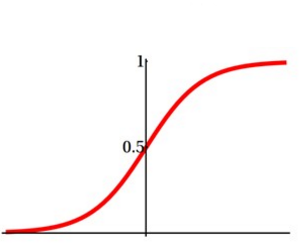
\includegraphics[width=5cm]{Bilder/Umsetzung/Sigmoid.PNG}}
\hfill
\subfigure[Tanh]{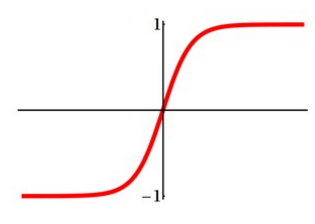
\includegraphics[width=5cm]{Bilder/Umsetzung/tanh.PNG}}
\hfill
\caption{Die Sigmoide Funktion und die Tanh Funktion im Vergleich}
\label{fig:sigtanh}
\end{figure}

\begin{equation}\formelentry{Sigmoide Funktion sowie Tanh Funktion}
(a)\ f(x)= \frac{1}{1+e^{-cx}}\ \ \ \ \ \ \ \ \ \ \ (b)\ f(x)= tanh(x)
\end{equation}


Aus der Tabelle \ref{tab:TRANSMSE} können die Ergebnisse dieses Optimierungsschrittes entnommen werden.


\begin{table}[H]
  \centering
  \begin{tabular}{|c|c|c|}
  \hline 
  \rule[0ex]{0pt}{2.5ex} Transferfunktion & Training-MSE & Test-MSE \\ 
  \hline 
  \rule[0ex]{0pt}{2.5ex} \textbf{Sigmoid} & $9.406 \cdot 10^{-4}$ & $0.001767$\\ 
  \hline 
  \rule[0ex]{0pt}{2.5ex} Tanh & $0.0103333$ & $0.044330$ \\ 
  \hline 
  \end{tabular} 
  \caption{Jeweilige Transferfunktionen \& korrespondierende MSE}
  \label{tab:TRANSMSE}
\end{table}

Man erkennt, dass es sich bei der bisher genutzten sigmoiden Funktion bereits um die beste Lösung handelt. Folglich wurde das KNN in dieser Hinsicht nicht weiter optimiert und die ursprüngliche Funktion wurde belassen.

\subsection{Wahl der optimalen Lernregel}
\label{subsection:Wahl der optimalen Lernregel}

Als letzten Schritt wurde die Lernregel des KNN optimiert. Innerhalb des Verfahrens der überwachten Lernens existieren mehrere Lernregeln, um das Netz zu trainieren. Die bekannteste Lernregel ist die Backpropagation-Lernregel. Diese Regel gibt es in mehreren Variationen. In dieser Seminararbeit werden zum einen das Grundverfahren sowie einige Variationen, namentlich das  "`Momentum Backpropagation"' sowie das "`Resilient Backpropagation"' beschrieben und untersucht. Anschließend wird das für die Anwendung am besten geeignete Verfahren ausgewählt\footnote{\Vgl\Zitat{Laemmel}, S. 225 f.}.

\begin{itemize}
\item \textbf{Backpropagation}:\\
Dies ist das klassische Fehlerrückführungsverfahren zum Anpassen der Verbindungsgewichte. Die Gewichtsveränderung erfolgt durch ein Fehlersignal, dass aus der Abweichung von tatsächlicher und prognostizierter Ausgabe berechnet wird. Die Gewichtsveränderung erfolgt hierbei schichtweise von den Ausgangs-Neuronen bis zu den Eingangs-Neuronen.

\item \textbf{Momentum Backpropagation}:\\
Dieses Verfahren fügt dem klassischen Verfahren einen Trägheitsterm hinzu, indem die Gewichtsveränderung zum Zeitpunkt $t-1$ berücksichtigt wird. Dieser Term kann einen Wert zwischen $0$ und $1$ annehmen. Umso größer dieser Term ist, umso stärker wir die vorhergehende Gewichtsveränderung berücksichtigt. Durch diesen Trägheitsterm wird die Wahrscheinlichkeit verringert, dass das KNN beim Training in ein lokales Minimum oszilliert und sich somit nicht weiter dem Idealwert approximieren kann. Auch die Wahl der Lernrate gestaltet sich hier weniger kritisch. 

\item \textbf{Resilient Propagation}:\\
Resilient heißt Federnd. Dieses Verfahren nutzt das Vorzeichen das Gradienten zum Zeitpunkt $t$ und entscheidet anhand dessen, ob das Gewicht vergrößert oder verkleinert werden muss. Der Betrag der Gewichtsveränderung wird jedoch unabhängig von der Richtung der Gewichtsänderung ermittelt.  Dadurch werden die typischen Probleme klassischer Gradientenabstiegsverfahren, wie sie beim klassischen Backpropagation sowie beim Momentum Backpropagation genutzt werden, gemindert.\footnote{\Vgl\Zitat{Valen}, S. 71}.

Die Formeln für Resilient Propagation lauten wie folgt:

\begin{equation}\formelentry{Formel zur Bestimmung der Art der Gewichtsänderung}
\Delta w_{ij}=\begin{cases} 
-\Delta_{ij} & falls S(t) > 0 \\ 
+\Delta_{ij} & falls S(t) < 0  \\ 
\pm 0       & sonst 
\end{cases}
\end{equation}

\begin{equation}\formelentry{Formel zur Bestimmung des Betrages der Gewichtsänderung}
\Delta_{ij}=\begin{cases} 
\Delta_{ij}(t-1)\cdot n^+ & falls S(t-1) \cdot S(t) > 0 \\ 
\Delta_{ij}(t-1)\cdot n^- & falls S(t-1) \cdot S(t) < 0 \\
\Delta_{ij}(t-1)       & sonst 
\end{cases}
\end{equation}


Solange das Vorzeichen des Gradienten negativ ist, wird das Vorzeichen des Gewichtes ebenfalls beibehalten und die Schrittweite und somit das Gewicht um einen konstanten Wert $n^{+}$ vergrößert. Somit können Plateaus besser überwunden werden.
Ändert sich das Vorzeichen des Gradienten von negativ auf positiv(was bedeutet, dass ein Minimum übersprungen wurde), so wird das Vorzeichen geändert und die Schrittweite um  einen fixen Faktor $n^{-}$ verringert. Somit werden Oszillationen verhindert.

Die Abbildung \ref{fig:RP} stellt das Vorgehen des Resilient Propagation Algorithmus grafisch dar\footnote{\Vgl\Zitat{Geith}, S. 71}.

\begin{figure}[H]
	\centering
	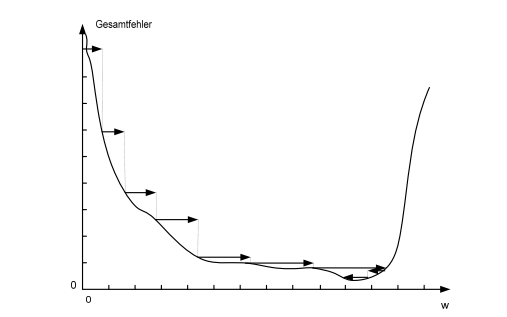
\includegraphics[width=10cm]{Bilder/Umsetzung/VisuResi.PNG}
	\caption{Visualisierung des Resilient Propagation Algorithmus}
	\label{fig:RP}
\end{figure}

\end{itemize}

Allen drei Lernregeln ist gemein, dass zur Bestimmung des Fehlers zwischen der prognostizierten und tatsächlichen Ausgabe der MSE benutzt werden kann. Die MSE-Formel würde in dem konkreten Fall der Anwendung wie folgt lauten:

\begin{equation}\formelentry{MSE zur Berechnung der Abweichung}
   \frac{1}{2}\sum^{n}_{i=1} (KT_{i} - KV_{i})^2
\end{equation}

Wobei $n$ für die Anzahl der Daten im Datensatz steht, $KT_i$ für den tatsächlichen Ausgabewert eines Datum $i$ steht und $KV_i$ für den korrespondierenden prognostizierten Ausgabewert eines Datums $i$ steht.

In der Tabelle \ref{tab:LERNregeln} kann das Ergebnis der Trainings- und Testdurchläufe mit den jeweiligen Lernregeln betrachtet werden.

\begin{table}[H]
  \centering
  \begin{tabular}{|c|c|c|}
  \hline 
  \rule[0ex]{0pt}{2.5ex} Lernregel & Training-MSE & Test-MSE \\ 
  \hline 
  \rule[0ex]{0pt}{2.5ex} Backpropagation & $9.325\cdot10^{-4}$ & $0.001636$ \\ 
  \hline 
  \rule[0ex]{0pt}{2.5ex} Momentum Backpropagation & $9.109\cdot10^{-4}$ & $0.001608$ \\ 
  \hline 
  \rule[0ex]{0pt}{2.5ex} \textbf{Resilient Propagation} & $8.89\cdot10^{-4}$ & $9.406\cdot10^{-4}$ \\ 
  \hline 
  \end{tabular} 
  \caption{Lernregeln \& jeweilige MSE}
  \label{tab:LERNregeln}
\end{table}

In der Regel liefert Resilient Propagation sehr gute Ergebnisse, dies ist auch hier der Fall. Wie man erkennen kann, ist das Resilient Propagation Verfahren  hier den anderen überlegen. Folglich wurde das KNN entsprechend optimiert und Resilient Propagation als Lernregel eingesetzt. Da es sich bei Resilient Propagation um eine adaptive Lernregel handelt und bei der Berechnung keine Lernrate benutzt handelt, muss diese auch nicht angegeben werden.

\section{Die endgültigen künstlichen neuronalen Netze}
\label{section:Die endgültigen künstlichen neuronalen Netze}

Nachdem das KNN zur Prognose des DAX erstellt und optimiert wurde, wurden diese Schritte in analoger weise für die KNN zur Prognose des Nikkei sowie zur Prognose des Dow Jones wiederholt.
Es stellte sich heraus, dass das optimale KNN für den DAX ebenfalls das Optimale KNN für den Nikkei und den Dow Jones darstellt. Das Endgültige Netz sowie dessen Parameter können aus der Tabelle \ref{tab:ENDconf} sowie aus der  Abbildung \ref{fig:ENDKNN} entnommen werden.

\begin{table}[H]
  \centering
  \begin{tabular}{|c|c|}
  \hline 
  \rule[0ex]{0pt}{2.5ex}  Topologie & 4-7-1 mit Bias\\ 
  \hline 
  \rule[0ex]{0pt}{2.5ex}  Lernregel & Resilient Propagation\\  
  \hline 
  \end{tabular} 
  \caption{Die jeweiligen Börsenkurse \& deren Endwerte}
  \label{tab:ENDconf}
\end{table}

\begin{figure}[H]
	\centering
	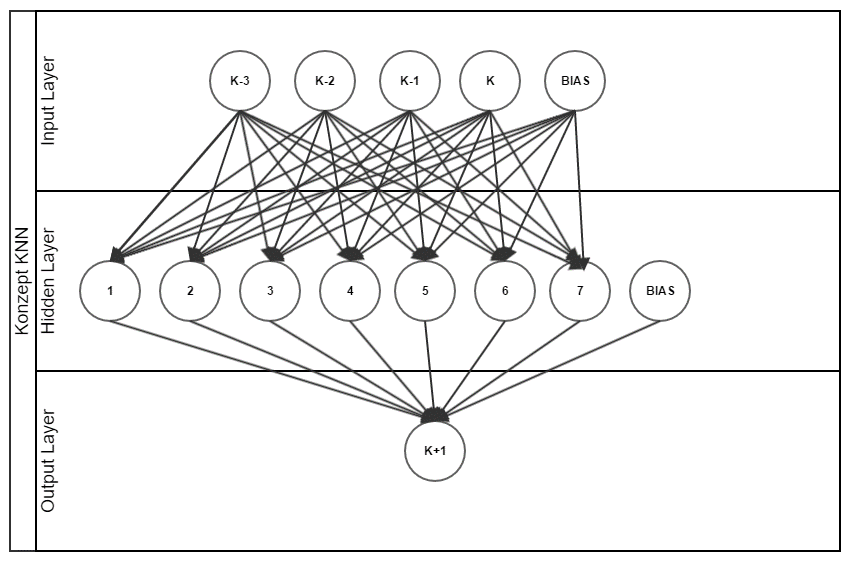
\includegraphics[width=10cm]{Bilder/Umsetzung/FertigKNN.PNG}
	\caption{Das endgültige KNN für alle Börsenkurse}
	\label{fig:ENDKNN}
\end{figure}

Die Tabelle \ref{tab:ENDval} zeigt die Trainings- sowie Testergebnisse der implementierten und optimierten KNN nach jeweils $200.000$ Trainingszyklen.

\begin{table}[H]
  \centering
  \begin{tabular}{|c|c|c|}
  \hline 
  \rule[0ex]{0pt}{2.5ex}  Börsenkurs & Training-MSE & Test-MSE\\ 
  \hline 
  \rule[0ex]{0pt}{2.5ex} DAX & $4.252\cdot10^{-5}$ & $4.820\cdot10^{-5}$  \\ 
  \hline 
  \rule[0ex]{0pt}{2.5ex} Nikkei & $1.350\cdot10^{-5}$ & $4.520\cdot10^{-5}$  \\ 
  \hline 
   \rule[0ex]{0pt}{2.5ex} Dow Jones & $6.672\cdot10^{-5}$ & $2.820\cdot10^{-4}$  \\ 
  \hline 
  \end{tabular} 
  \caption{Die endgültigen Parameter für alle KNN}
  \label{tab:ENDval}
\end{table}
